% ---- Introduction (shared; counts towards the 3000-word limit) ----
\section{Introduction}

Titan, Saturn's largest moon, is among the most compelling astrobiological targets in the Solar
System. The emergence of life as we understand it requires three ingredients in one place: a liquid
solvent, a supply of organic building blocks spanning the biogenic elements (CHNOPS), and a sustained
source of energy \citep{Maruyama2019}. Titan is the only body besides Earth known to host stable
surface liquids -- though its lakes and seas are methane and ethane rather than water -- and the only
moon with a dense, organic-rich atmosphere \citep{Sohl2014}. Photochemistry in that atmosphere
generates complex nitrogen-bearing organics, or tholins, along with prebiotic feedstock molecules such
as hydrogen cyanide \citep{Raulin2008}. Beneath roughly 100\,km of water ice, Cassini gravity and
rotation measurements inferred a global subsurface water ocean \citep{Iess2012, Durante2019}, an
environment that would satisfy the solvent requirement directly.

The central obstacle to Titan's habitability is not a shortage of ingredients but their separation.
Organics accumulate at the surface and in the atmosphere, while liquid water lies kilometres below an
insulating ice shell; the two rarely meet. Moreover, the very existence of the ocean is now contested:
recent re-analyses argue that Titan's measured tidal dissipation is too large to be compatible with a
decoupled liquid layer \citep{Petricca2025}, while others infer only a low-density ocean from a
reduced Love number \citep{Goossens2024}. Whether, where, and when Titan brings solvent, organics, and
energy together therefore remains genuinely open.

This report addresses that overarching question through five complementary, cross-disciplinary studies
that together span Titan from its silicate core to its upper atmosphere, following the layered
structure of Figure~\ref{fig:crosssection}. Working outward from the deep interior, Crick
\citep{Crick2026} models tidal heating and the thermal survival of the subsurface ocean; Nicolaides
\citep{Nicolaides2026} quantifies impact-generated melt production in the ice shell over Titan's
bombardment history; Castlevetro \citep{Castlevetro2026} simulates prebiotic chemistry within the
transient brine pockets those impacts create; and Islam Rahim \citep{IslamRahim2026} characterises
longitudinal and temporal structure in the organic-rich atmosphere. Meadows \citep{Meadows2026} then
draws these threads together at the surface, mapping the probability of habitability across the globe
and through geological time. Impact cratering emerges as a connective process linking these layers,
since it can excavate liquid water, mix in surface and cometary organics, and deliver both to depth
\citep{Thompson1992, Neish2024}.

\begin{figure}[htbp]
  \centering
  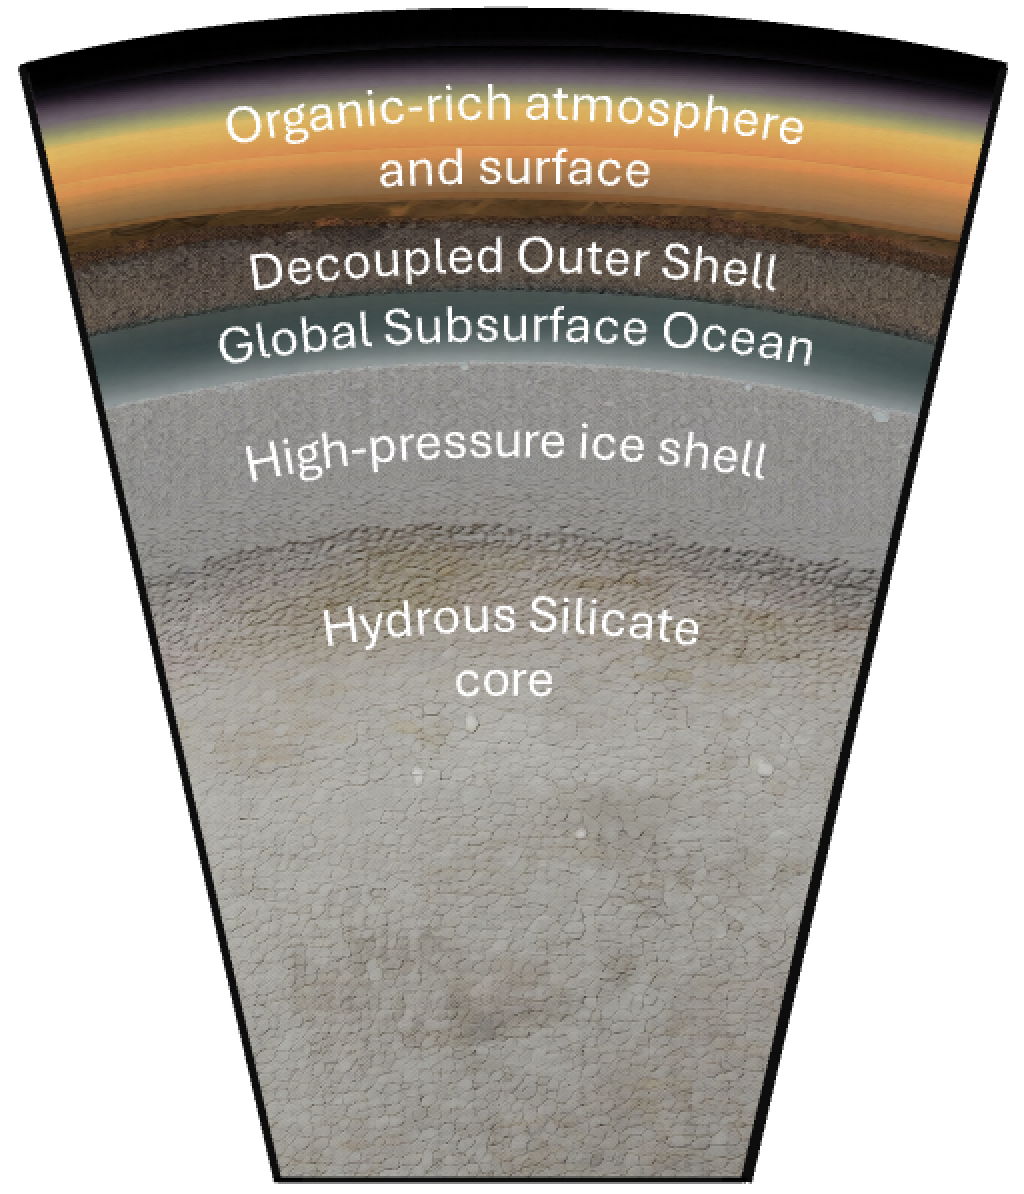
\includegraphics[width=0.5\linewidth]{images/titan_cross_section.png}
  \caption{Schematic cross-section of Titan's interior, from the hydrous silicate core through the
    high-pressure ice shell, the (contested) global subsurface ocean, and the decoupled outer ice
    shell, to the organic-rich surface and atmosphere. This report is organised around these layers:
    each of the five studies addresses habitability within one layer, or the exchange of material and
    energy between them, working from the interior outward. The figure provides the shared spatial
    frame for the summaries that follow.}
  \label{fig:crosssection}
\end{figure}

A second unifying theme is time. Titan's habitability is not static: the bombardment flux, the interior
thermal state, the surface insolation, and the atmosphere have all evolved from the Late Heavy
Bombardment towards the far future, when a red-giant Sun will warm the surface. The NASA Dragonfly
mission, arriving in 2034, will test many of these ideas directly at Selk crater \citep{Lorenz2021Landing}. In
the sections that follow we summarise the key insight from each study in turn, before synthesising them
into a combined outlook for Titan's habitability.
